\chapter{Navier Stokes as Inference on the Solution Manifold}
\label{ch:nsinference}

\section{The inverse direction}

The derivation of Chapter~\ref{ch:hydro} runs from particles to fluids and from the past to the future. Data run the other way. A meteorologist observes winds and pressures at scattered stations and wants the state of the atmosphere six hours ago, from which a forecast can be launched. An engineer measures velocities in a pipe by magnetic resonance and wants the inflow condition and the wall shape. A physicist observes a turbulent field and wants the forcing that maintains it. In every case the unknown is an initial or boundary condition, or a parameter, of a known evolution equation, and the observations are noisy and incomplete functions of the solution. Bayes' rule turns each of these problems into a posterior distribution for the unknown. The solution map carries that posterior to a distribution on space time fields that satisfy the equation, a measure on the solution manifold of Proposition~\ref{prop:solution_manifold}, and this is why the manifold is the right object for inference.

\section{Setting}

Let $\T^d = (\R/2\pi\Z)^d$ with $d\in\{2,3\}$, and let $\Phi_t$ denote the solution map of the incompressible Navier Stokes equations
\[
\partial_tu+u\cdot\nabla u+\nabla p = \nu\Delta u+f,\qquad\nabla\cdot u = 0,
\]
on a space $X$ of divergence free, mean zero fields. In two dimensions $\Phi_t$ is globally defined and smooth for initial data in $L^2$, by the classical theory of Leray, Ladyzhenskaya and Lions. In three dimensions it is defined on a maximal interval that may be finite. Observations are taken as in \eqref{eq:observation_model}, for example point values or Fourier coefficients of $u(t_j)$ with Gaussian noise of level $\delta$. The unknown $\theta = u(0)$, possibly together with $\nu$ and $f$, is given a Gaussian prior on a Sobolev space $H^\alpha$, and the posterior is defined by Bayes' rule. When the observation space is finite dimensional and the forward map grows at most polynomially in the norm of the unknown, the posterior depends Lipschitz continuously on the data in the Hellinger distance, by the theory of Stuart~\cite{stuart2010}, which we state as Theorem~\ref{thm:stuart_wellposed}.

Two structural facts govern everything. The forward map is injective in two dimensions: by the backward uniqueness theorem of Bardos and Tartar~\cite{bardostartar1973}, two solutions that agree at time $T$ agree at all earlier times. And its inverse is unstable: the dissipation $\nu\Delta$ damps the Fourier mode $k$ at the rate $e^{-\nu|k|^2t}$, so high frequencies of the initial condition leave only exponentially faint traces in the data. This combination is the setting in which priors matter and in which Bayesian inference is more than a reformulation of regularization.

\section{The linear case solved exactly}\label{sec:linearheat}

Linearize about the zero solution and drop the nonlinearity. The heat equation $\partial_tu = \Delta u$ on $(0,\pi)$ with Dirichlet conditions diagonalizes in the sine basis $\phi_k(x) = \sqrt{2/\pi}\sin(kx)$. Writing $\theta = \sum_k\theta_k\phi_k$ for the initial condition and observing the solution at time $T$ in white noise of level $\delta$ gives the sequence model
\[
y_k = e^{-k^2T}\theta_k+\delta\varepsilon_k,\qquad\varepsilon_k\sim N(0,1)\text{ independent}.
\]
With the prior $\theta_k\sim N(0,\lambda_k)$ independently, the posterior is Gaussian and diagonal:
\[
\theta_k\mid y\sim N\Big(\frac{v_ke^{-k^2T}}{\delta^2}y_k,\;v_k\Big),\qquad v_k = \Big(\frac{e^{-2k^2T}}{\delta^2}+\frac1{\lambda_k}\Big)^{-1}.
\]
Mode $k$ is learned when $e^{-k^2T}\gg\delta/\sqrt{\lambda_k}$, that is, for $k\lesssim K_\delta = \sqrt{\log(1/\delta)/T}$ up to lower order terms, and is otherwise left at its prior. Figure~\ref{fig:heat_inverse} shows this for $T = 0.05$, $\delta = 0.002$ and $\lambda_k = k^{-3}$. Here $K_\delta\approx11.1$, but the lower order terms matter: the equation $e^{-k^2T} = \delta/\sqrt{\lambda_k}$ has the solution $k\approx7.9$, because the prior variance decays with $k$. The ratio of posterior to prior standard deviation is below $0.2$ for $k\leq6$, crosses one half near $k = 7.3$ and exceeds $0.95$ for $k\geq9$.

\begin{figure}[t]
\centering
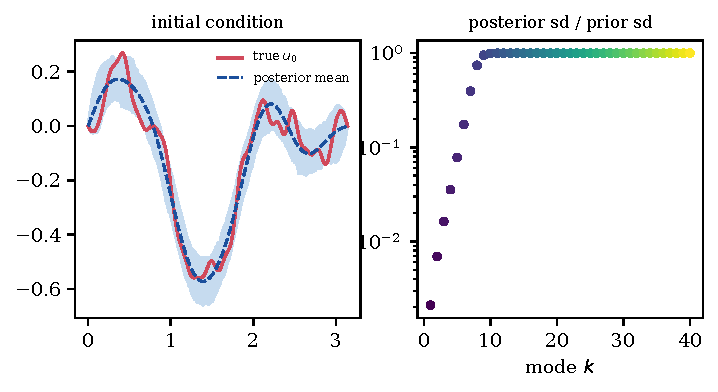
\includegraphics[width=\textwidth]{heat_inverse}
\caption{Inferring the initial condition of the heat equation from observations at time $T = 0.05$ with noise level $\delta = 0.002$, prior variances $\lambda_k = k^{-3}$ and $40$ Fourier modes. The truth is a draw from the prior. Left, truth, posterior mean and pointwise $90\%$ band computed from $200$ posterior draws; right, ratio of posterior to prior standard deviation by Fourier mode.}
\label{fig:heat_inverse}
\end{figure}

\begin{theorem}[Rates for the backward heat equation]
\label{thm:heat_rates}
Suppose $\lambda_k = k^{-1-2\alpha}$ with $\alpha>0$ and the true initial condition $\theta_0$ lies in a Sobolev ball of smoothness $\beta>0$. Then the posterior contracts in $L^2$ around the truth at the rate $(\log(1/\delta))^{-\min(\alpha,\beta)/2}$ up to constants, uniformly over the ball, and this is the minimax rate when $\alpha\geq\beta$. For a linear functional $L\theta = \sum_kl_k\theta_k$ whose coefficients satisfy $\sum_k|l_k|\,e^{2k^2T}k^{1+2\alpha}<\infty$ and $S = \sum_kl_k^2e^{2k^2T}>0$, let $\hat L = \sum_kl_ke^{k^2T}y_k$ be the unbiased estimator. Let $\Theta_B = \{\theta_0:\sup_k|\theta_{0,k}|\leq B\}$, a set that contains every Sobolev ball of smoothness $\beta\geq0$ and radius at most $B$, and let $\P_{\theta_0}$ be the law of the data under the truth $\theta_0$. Then for every $B>0$ and $\eta>0$, as $\delta\to0$,
\[
\sup_{\theta_0\in\Theta_B}\P_{\theta_0}\Big(\big\|\Pi\big((L\theta-\hat L)/\delta\in\cdot\mid y\big)-N(0,S)\big\|_{TV}>\eta\Big)\to0,
\]
and $(\hat L-L\theta_0)/\delta\sim N(0,S)$ exactly under the truth $\theta_0$. A Bernstein von Mises theorem therefore holds for $L\theta$, and equal tailed posterior credible intervals for $L\theta$ are asymptotically exact confidence intervals, uniformly over $\Theta_B$.
\end{theorem}

\begin{proof}
The $L^2$ rate is Theorem~2.1 of Knapik, van der Vaart and van Zanten~\cite{knapik2013}, with their prior scale equal to one and $n = \delta^{-2}$, and we do not repeat its proof. The mechanism is that modes $k\leq K_\delta$ are estimated with error of order $\delta e^{k^2T}$ while modes $k>K_\delta$ are left at the prior, and the tail $\sum_{k>K_\delta}(\theta_{0,k}^2+\lambda_k)$ is of order $K_\delta^{-2\min(\alpha,\beta)}$ with $K_\delta\asymp(\log(1/\delta))^{1/2}$.

For the functional, write $r_k = \delta^2e^{2k^2T}/(\lambda_k+\delta^2e^{2k^2T})\in[0,1]$, so that $v_k = \delta^2e^{2k^2T}(1-r_k)$ and the posterior mean of $\theta_k$ is $m_k = (1-r_k)e^{k^2T}y_k$. The posterior of $L\theta$ is Gaussian with mean $\sum_kl_km_k$ and variance $\sum_kl_k^2v_k = \delta^2\sum_kl_k^2e^{2k^2T}(1-r_k)$. Since $r_k\to0$ for each $k$ as $\delta\to0$ and $0\leq r_k\leq1$, dominated convergence gives $\sum_kl_k^2v_k = \delta^2(S+o(1))$, using $\sum_kl_k^2e^{2k^2T}\leq\sup_k|l_k|e^{k^2T}\sum_k|l_k|e^{k^2T}<\infty$. For the centering, substituting $y_k = e^{-k^2T}\theta_{0,k}+\delta\varepsilon_k$ under the truth,
\[
\sum_kl_km_k-\hat L = -\sum_kl_kr_k\theta_{0,k}-\delta\sum_kl_kr_ke^{k^2T}\varepsilon_k.
\]
The first term is bounded by $\sup_k|\theta_{0,k}|\sum_k|l_k|r_k\leq\delta^2B\sum_k|l_k|e^{2k^2T}\lambda_k^{-1} = O(\delta^2)$ uniformly over $\Theta_B$ by the summability assumption, since $\lambda_k^{-1} = k^{1+2\alpha}$. The second term is centered Gaussian with variance $\delta^2\sum_kl_k^2r_k^2e^{2k^2T} = o(\delta^2)$ by dominated convergence, a variance that does not depend on $\theta_0$. Hence $(\sum_kl_km_k-\hat L)/\delta\to0$ in $\P_{\theta_0}$ probability, uniformly over $\Theta_B$, and the posterior of $(L\theta-\hat L)/\delta$ is a Gaussian whose mean tends to zero and whose variance tends to $S>0$; convergence of Gaussian laws in total variation follows from convergence of their parameters. Under the truth, $\hat L-L\theta_0 = \delta\sum_kl_ke^{k^2T}\varepsilon_k\sim N(0,\delta^2S)$ exactly. An equal tailed credible interval for $L\theta$ therefore has endpoints $\hat L\pm z\delta\sqrt S+o(\delta)$ in probability, uniformly over $\Theta_B$, where $z$ is a normal quantile, and its coverage tends to the nominal level.
\end{proof}

The first part of the theorem is due to Knapik, van der Vaart and van Zanten~\cite{knapik2013}, who also show that credible balls for the whole initial condition have asymptotic coverage zero when the prior is smoother than the truth and coverage one, with a radius larger than that of a confidence ball by a diverging factor, when it is rougher. For linear functionals whose coefficients decay only polynomially they show that credible intervals have asymptotic coverage zero or one, so that no Bernstein von Mises theorem holds for them. The second part of the theorem is proved above. For the direct white noise model, Bernstein von Mises theorems for linear and nonlinear functionals are due to Castillo and Nickl~\cite{castillonickl2013}. The reconstruction of the whole initial condition is possible only at logarithmic rates; no method can do better uniformly over a Sobolev ball. But smooth functionals of the initial condition, those whose coefficients decay faster than the damping, are estimable at the parametric rate, and the Bayesian posterior quantifies their uncertainty correctly. Inference on the solution manifold is therefore an exercise in choosing the questions the data can answer.

\section{The nonlinear theory}

For nonlinear forward maps the corresponding theory was developed by Nickl and coauthors and is presented in Nickl's lectures~\cite{nickl2023book}. Its architecture has three components.

The first is a \emph{forward regularity} estimate: the map $\mathcal{G}:\theta\mapsto(\mathcal{O}_j\Phi_{t_j}\theta)_j$ is Lipschitz, with polynomial growth of the constant, from the parameter space to the observation space. For Navier Stokes in two dimensions this follows from energy estimates.

The second is a \emph{stability} estimate in the reverse direction: $\|\theta-\theta'\|_{H^{-s}}\leq\chi(\|\mathcal{G}(\theta)-\mathcal{G}(\theta')\|)$ for some modulus $\chi$, valid on bounded sets of a smoother space. For parabolic problems observed only at positive times $\chi$ is typically logarithmic, as in the linear case. Combined with posterior contraction in the observation space, which holds at the usual rates by general theory for Gaussian priors rescaled with the sample size, stability transfers contraction to the parameter.

The third is \emph{computation}. Nickl and Wang~\cite{nicklwang2024} showed, for one model, that a lower bound on the Fisher information operator called gradient stability makes the log likelihood strongly concave near the truth, and that a Langevin type algorithm, initialized by a suitable estimator and run on a surrogate of the posterior, then samples from it to given accuracy in a number of steps polynomial in the dimension and the sample size (Section~\ref{sec:gradstab}).

For time evolution equations, Nickl and Titi~\cite{nickltiti2024} proved posterior consistency for the two dimensional Navier Stokes equations, with inverse logarithmic rates for the initial condition, and showed that in general no faster rate is possible when the observation times are sampled from a window bounded away from zero. When the observations are spread over space and time starting at time zero, the stability estimate improves and the posterior contracts at a polynomial rate in the number $N$ of observations~\cite{konennickl2026}. For such observations Nickl proved a Bernstein von Mises theorem for reaction diffusion equations~\cite{nicklbvm2024}, and Konen and Nickl proved one for Navier Stokes~\cite{konennickl2026}: the posterior law of the trajectory, centered at the posterior mean and scaled by $\sqrt N$, is close to a Gaussian law in Wasserstein distance for the supremum norm over any time window bounded away from zero. Our own work~\cite{polsonsokolov2026manifold} combines this theory with simulation based computation, as we now describe and as Chapters~\ref{ch:manifold} to~\ref{ch:examples} treat in detail.

\section{Gradient stability and polynomial time sampling}
\label{sec:gradstab}

\subsubsection{The computational question} The posterior of a nonlinear partial differential equation inverse problem is a density on $\R^D$ with $D$ large, and it is not log concave, because the forward map is nonlinear and enters the log likelihood through a square. A Markov chain can take a time exponential in $D$ to mix, and since the posterior becomes spiked as $N$ grows, iterative algorithms can take a time exponential in $N$ to leave a neighborhood of a local optimum~\cite{nicklwang2024}. The preconditioned Crank Nicolson chain of Section~\ref{sec:dimrobust} has a spectral gap independent of the discretization~\cite{hairer2014}, but the bound is not quantitative in $N$ and $D$~\cite{nicklwang2024}. The question is when the posterior mean can be computed to accuracy $\varepsilon$ in a number of steps polynomial in $N$, $D$ and $\varepsilon^{-1}$, with high probability under the data. Nickl and Wang answer it for one model, under a hypothesis on the forward map called gradient stability. We ask where it holds, above all for the two dimensional Navier Stokes equations. Numbers of theorems, lemmas and equations of Nickl and Wang, of Konen and Nickl and of Castre and Nickl refer to the arXiv versions 2009.05298v2, 2507.18279v2 and 2601.10326v1.

\subsubsection{Setting} We use the notation of Nickl and Wang, with the forward map written $\mathcal{G}$, $P^X$ the uniform probability measure on a bounded set $\mathcal{X}$ and $\|\cdot\|_{L^2}$ the norm of $L^2(P^X)$. For $\theta\in\R^D$, the coefficients of the unknown in the first $D$ basis elements, the data $Z_i=(Y_i,X_i)$ satisfy
\begin{equation}\label{eq:gs_model}
Y_i=\mathcal{G}(\theta)(X_i)+\varepsilon_i,\qquad X_i\sim P^X,\quad\varepsilon_i\sim N(0,1),\qquad i=1,\dots,N,
\end{equation}
all independent, under a truth $\theta_0$ that need not lie in $\R^D$ (we write $\P_{\theta_0}^N$ and $\E_{\theta_0}$). For an evolution equation, $\mathcal{X}=[0,T]\times\T^d$ and $\mathcal{G}(\theta)(t,x)$ is the solution at time $t$ and position $x$. This is the observation model~\eqref{eq:observation_model} with $\mathcal{O}_j$ the evaluation at a random point of space and time and unit noise. With $\ell(\theta,Z)=-\frac12(Y-\mathcal{G}(\theta)(X))^2$, $\ell_N(\theta)=\sum_{i\le N}\ell(\theta,Z_i)$ and a Gaussian prior $N(0,\Sigma)$ with density $\pi$, the posterior $\Pi(\cdot\mid Z)$ has density proportional to $e^{\ell_N}\pi=e^{-H}$, where $H(\theta)=-\ell_N(\theta)+\frac12\theta^\top\Sigma^{-1}\theta$.

\subsubsection{Gradient stability} Differentiating $\ell$ twice and using $\E_{\theta_0}[Y\mid X]=\mathcal{G}(\theta_0)(X)$ gives, for every $v\in\R^D$,
\begin{equation}\label{eq:gs_hess}
\begin{aligned}
v^\top\E_{\theta_0}\big[-\nabla^2\ell(\theta,Z)\big]v={}&\big\|v^\top\nabla\mathcal{G}(\theta)\big\|_{L^2}^2\\
&+\big\langle\mathcal{G}(\theta)-\mathcal{G}(\theta_0),\,v^\top\nabla^2\mathcal{G}(\theta)v\big\rangle_{L^2}.
\end{aligned}
\end{equation}
At $\theta=\theta_0$, when this lies in $\R^D$, the second term vanishes and the matrix is the Fisher information $I(\theta_0)=\E_X[\nabla\mathcal{G}(\theta_0)(X)\nabla\mathcal{G}(\theta_0)(X)^\top]$ of one observation. The expected Hessian of $-\ell_N$ is $N$ times this matrix, so a lower bound on its smallest eigenvalue says that the data are informative in every direction, and by~\eqref{eq:gs_hess} it follows from an injectivity estimate for the gradient.

\begin{definition}[Gradient stability]\label{def:gs_stab}
Let $B\subset\R^D$ and $c>0$. The forward map $\mathcal{G}$ is gradient stable on $B$ with constant $c$ if $\theta\mapsto\mathcal{G}(\theta)(x)$ is differentiable on $B$ for every $x$ and
\begin{equation}\label{eq:gs_stab}
\big\|v^\top\nabla\mathcal{G}(\theta)\big\|_{L^2}\ge c\,|v|\qquad\text{for all }\theta\in B\text{ and }v\in\R^D.
\end{equation}
\end{definition}

Nickl and Wang take $B=\{\theta:|\theta-\theta^*|_1<\eta\}$, with $\theta^*\in\R^D$ a centering point (the projection of $\theta_0$) and $|\theta|_1^2=\theta^\top M\theta$ for a symmetric positive definite matrix $M$. The difficulty lies in the dependence of the constant $c$ on $D$, which Castre and Nickl~\cite{castrenickl2026} make explicit. What enters the theorem is the local curvature condition
\begin{equation}\label{eq:gs_curv}
\inf_{\theta\in B}\lambda_{\min}\big(\E_{\theta_0}[-\nabla^2\ell(\theta,Z)]\big)\ge c_{\min}>0 .
\end{equation}
It follows from~\eqref{eq:gs_stab} by a line that we add. If $k_0$ and $k_2$ bound the supremum norms of $\mathcal{G}(\theta)-\mathcal{G}(\theta_0)$ and of $\|\nabla^2\mathcal{G}(\theta)\|_{\mathrm{op}}$ over $B$, the second term of~\eqref{eq:gs_hess} is at least $-k_0k_2|v|^2$ by the Cauchy Schwarz inequality, so gradient stability with constant $c$ and $k_0k_2\le c^2/2$ give~\eqref{eq:gs_curv} with $c_{\min}=c^2/2$.

The Bernstein von Mises theory of this chapter rests on invertibility of the information operator, the derivative of the forward map composed with its adjoint, between Sobolev spaces, which Konen and Nickl~\cite{konennickl2026} prove for the two dimensional Navier Stokes equations. Gradient stability is its quantitative counterpart on $D$ coordinates. It is local, and hence weaker than the Polyak \L{}ojasiewicz condition of nonconvex optimization, a global lower bound on the squared gradient by the suboptimality, as Nickl and Wang remark.

\subsubsection{The theorem of Nickl and Wang} \emph{Local regularity} asks that $\mathcal{G}(\theta)(x)$ be twice continuously differentiable in $\theta\in B$, with $\mathcal{G}(\theta)-\mathcal{G}(\theta_0)$, $\nabla\mathcal{G}(\theta)$ and $\nabla^2\mathcal{G}(\theta)$ bounded in the supremum norm over $x$ by $k_0,k_1,k_2$ and Lipschitz in $\theta$ for $|\cdot|_1$ with constants $m_0,m_1,m_2$. \emph{Local curvature} asks for~\eqref{eq:gs_curv} and for a bound $c_{\max}\ge c_{\min}$ on the expected log likelihood and its first two derivatives over $B$. The algorithm needs an initializer $\theta_{\mathrm{init}}\in\R^D$ computed from the data and a surrogate $\tilde\ell_N=\alpha_\eta\ell_N-Kg_\eta$ of the log likelihood. Here $\alpha_\eta$ is a smooth cutoff in $|\theta-\theta_{\mathrm{init}}|_1/\eta$, $g_\eta$ is a convex penalty that vanishes for $|\theta-\theta_{\mathrm{init}}|_1\le\eta/2$, and $K>0$ is large. The surrogate posterior $\tilde\Pi(\cdot\mid Z)$ has density proportional to $e^{\tilde\ell_N}\pi$, and the unadjusted Langevin algorithm (ULA) for it, with step size $\gamma>0$ and independent $\xi_k\sim N(0,I_D)$, is
\begin{equation}\label{eq:gs_ula}
\vartheta_0=\theta_{\mathrm{init}},\qquad\vartheta_{k+1}=\vartheta_k+\gamma\big(\nabla\tilde\ell_N(\vartheta_k)-\Sigma^{-1}\vartheta_k\big)+\sqrt{2\gamma}\,\xi_{k+1}.
\end{equation}
Three events enter. On $E_{\mathrm{conv}}$, $\lambda_{\min}(-\nabla^2\ell_N(\theta))\ge Nc_{\min}/2$ and $|\ell_N|+|\nabla\ell_N|+\|\nabla^2\ell_N\|_{\mathrm{op}}\le N(5c_{\max}+1)$ for all $\theta\in B$. Further $E_{\mathrm{init}}=\{|\theta_{\mathrm{init}}-\theta^*|_1\le\eta/8\}$ and $E_{\mathrm{wass}}(\rho)=\{W_2^2(\Pi(\cdot\mid Z),\tilde\Pi(\cdot\mid Z))\le\rho/2\}$, where $W_2$ is the Wasserstein distance of Chapter~\ref{ch:entropy}.

\begin{theorem}[Nickl and Wang, in simplified form]\label{thm:gs_main}
Let the data follow~\eqref{eq:gs_model}, let the prior be $N(0,\Sigma)$ and let local regularity and local curvature hold on $B$ with $\eta\in(0,1]$. Let $R_N$ be the quantity of equation~(45) of~\cite{nicklwang2024}, a universal constant times $N$ times the minimum of eight ratios of the constants above; in particular $R_N\le CNc_{\min}^2/(k_1^2+k_0k_2+k_2)^2$.
\begin{enumerate}[label=(\roman*),nosep]
\item If $D\le R_N$, then $\P_{\theta_0}^N(E_{\mathrm{conv}})\ge1-32e^{-R_N}-e^{-N/8}$.
\item Let $D\le R_N$, $K\ge CN(c_{\max}+1)(1+\lambda_{\max}(M)\eta^{-2})/\lambda_{\min}(M)$, $m=\frac12Nc_{\min}+\lambda_{\min}(\Sigma^{-1})$ and $\Lambda=7K\lambda_{\max}(M)+\lambda_{\max}(\Sigma^{-1})$. Then for every $\rho>0$, $0<\gamma\le1/(m+\Lambda)$ and $k\ge0$, on $E=E_{\mathrm{conv}}\cap E_{\mathrm{init}}\cap E_{\mathrm{wass}}(\rho)$,
\begin{equation}\label{eq:gs_w2}
W_2^2\big(\Law(\vartheta_k),\Pi(\cdot\mid Z)\big)\le\rho+b(\gamma)+4\Big(\tau+\frac Dm\Big)\Big(1-\frac{\gamma m}2\Big)^k,
\end{equation}
where $b(\gamma)=c_1(\gamma D\Lambda^2m^{-2}+\gamma^2D\Lambda^4m^{-3})$, $\tau=c_2\kappa(\Sigma)(1+\eta^2/\lambda_{\min}(M)+R^2)$ for any $R\ge|\theta^*|$, $\kappa(\Sigma)=\lambda_{\max}(\Sigma)/\lambda_{\min}(\Sigma)$, and $C,c_1,c_2$ are universal constants.
\end{enumerate}
\end{theorem}

Part (i) is Lemma~3.4 and part (ii) is Proposition~3.6 with Theorem~3.7 of~\cite{nicklwang2024}. Their Theorem~3.7 allows $0<\gamma\le1/\Lambda$; its proof applies, through their Proposition~A.4, Theorem~5 of Durmus and Moulines~\cite{durmusmoulines2019}, which is proved for $\gamma\le1/(m+\Lambda)$, and we state (ii) in that range. Since $m\le\Lambda$, this costs at most a factor $2$ in the step, and for large $N$ the range contains the step sizes used below. We quote the theorem without proof. The theorem does not say that $E_{\mathrm{init}}$ and $E_{\mathrm{wass}}(\rho)$ have high probability. Bounding their probability, Nickl and Wang write, `may pose a formidable challenge in its own right', and they do it for the Schr\"odinger equation only.

\begin{corollary}[Posterior mean and mode]\label{cor:gs_mean}
In the setting of Theorem~\ref{thm:gs_main}(ii) let $\bar\vartheta$ be the average of $\vartheta_{J_{\mathrm{in}}+1},\dots,\vartheta_{J_{\mathrm{in}}+J}$.
\begin{enumerate}[label=(\alph*),nosep]
\item There are constants $c_3,c_5>0$ such that on $E$, for $t\ge\sqrt8\,(\rho+b(\gamma))^{1/2}$, $mJ\gamma\ge1$ and $J_{\mathrm{in}}\ge(c_3/m\gamma)\log\big(1+(\rho+b(\gamma))^{-1}+\tau+D/m\big)$, $\P_{\theta_{\mathrm{init}}}(|\bar\vartheta-\E^\Pi[\theta\mid Z]|\ge t)\le2D\exp(-c_5t^2m^2J\gamma/D)$.
\item If the posterior density has a maximizer and every maximizer lies in $\{|\theta-\theta^*|_1\le3\eta/8\}$, then on $E_{\mathrm{conv}}\cap E_{\mathrm{init}}$ the posterior has a unique mode, and gradient ascent on the logarithm of the surrogate density from $\theta_{\mathrm{init}}$ with step $(2\Lambda)^{-1}$ converges to it, with squared error at most a constant, which depends on the data, times $(1-m/(2\Lambda))^k$.
\end{enumerate}
\end{corollary}

Part (a) is Corollary~3.9 of~\cite{nicklwang2024}, quoted without proof, with the factor $1+1/(mJ\gamma)\le2$ in the exponent of their bound absorbed in $c_5$. Part (b) is our formulation of their Proposition~A.2 and of the argument after their equation~(158), and the argument is short. On $E_{\mathrm{conv}}\cap E_{\mathrm{init}}$ the surrogate $\tilde\ell_N$ and $\ell_N$ have the same gradient on the ball of (b), so a maximizer of the posterior density is a critical point of the logarithm of the surrogate density, which is strongly concave and has one critical point only. Proposition~A.2 is the geometric rate of gradient descent for a function whose Hessian lies between $mI$ and $\Lambda I$. With $\rho\le\varepsilon^2/16$ and $b(\gamma)\le\varepsilon^2/16$ the threshold for $t$ is at most $\varepsilon$, and the number of steps is polynomial in $N$, $D$, $m^{-1}$, $\Lambda$ and $\varepsilon^{-1}$.

\subsubsection{The Schr\"odinger equation} Nickl and Wang prove $E_{\mathrm{init}}$ and $E_{\mathrm{wass}}$ for the steady state Schr\"odinger equation $\frac12\Delta u-fu=0$ on a bounded smooth domain $\mathcal{O}\subset\R^d$, $d\le3$, of unit volume, with boundary values $u=g$, an elliptic boundary value problem. The unknown is $f_\theta=\Phi\circ F_\theta$, where $F_\theta=\sum_{k\le D}\theta_ke_k$ in the eigenfunctions of the Dirichlet Laplacian, with eigenvalues $\lambda_k$, and $\Phi$ is a regular link function. The forward map is $\mathcal{G}(\theta)=u_{f_\theta}$, the design is uniform on $\mathcal{O}$, and the prior is $N(0,N^{-d/(2\alpha+d)}\Lambda_\alpha^{-1})$ with $\Lambda_\alpha=\diag(\lambda_1^\alpha,\dots,\lambda_D^\alpha)$ and an integer $\alpha>6$.

\begin{theorem}[Nickl and Wang, Schr\"odinger equation, in simplified form]\label{thm:gs_schr}
Let $\theta_0$ satisfy $\sum_k\lambda_k^\alpha\theta_{0,k}^2<\infty$, and for some constants $c_0>0$ and $0<c_0'<1/2$ let $D\le c_0N^{d/(2\alpha+d)}$ and $\|\mathcal{G}(\theta_{0,D})-\mathcal{G}(\theta_0)\|_{L^2}\le c_0'N^{-\alpha/(2\alpha+d)}$, where $\theta_{0,D}$ is the projection of $\theta_0$ onto $\R^D$. Run~\eqref{eq:gs_ula} with $M=I$, $\theta^*=\theta_{0,D}$, $\eta=D^{-4/d}/\log N$, $K=ND^{8/d}(\log N)^3$, $\gamma\le(ND^{8/d}(\log N)^4)^{-1}$ and the initializer of Theorem~B.6 of~\cite{nicklwang2024}. On events of probability at least $1-ce^{-c'N^{d/(2\alpha+d)}}$, for every $P>0$ and $\varepsilon\ge N^{-P}$:
\begin{enumerate}[label=(\roman*),nosep]
\item there are a step size and a number of steps $O(N^{b_1}D^{b_2}\varepsilon^{-b_3})$ after which $W_2(\Law(\vartheta_k),\Pi(\cdot\mid Z))\le\varepsilon$, and averaging the chain computes the posterior mean to accuracy $\varepsilon$ at a cost of the same form; the exponents $b_1,b_2,b_3>0$ are not specified and may differ between the two statements;
\item the posterior has a unique mode, and gradient ascent on the logarithm of the surrogate density with step size $(ND^{8/d}(\log N)^4)^{-1}$ comes within $cN^{-\alpha^2/((2\alpha+d)(\alpha+2))}$ of $\theta_0$ in $\ell^2$ after $O(D^{12/d}(\log N)^5)$ iterations.
\end{enumerate}
\end{theorem}

We quote the theorem without proof. It collects Theorem~1.1 and Theorems~2.5, 2.7 and~2.8 of~\cite{nicklwang2024}, which are Theorem~\ref{thm:gs_main} and Corollary~\ref{cor:gs_mean} with the scalings of their Proposition~4.1, together with their Theorems~B.6 and~4.14 for $E_{\mathrm{init}}$ and $E_{\mathrm{wass}}$. The scalings are $k_0\simeq k_1\simeq1$, $k_2\simeq m_0\simeq m_1\simeq D^{2/d}$, $m_2\simeq D^{4/d}$, $c_{\max}\simeq1$ and, from an elliptic stability estimate, $c_{\min}\simeq D^{-4/d}$. Then $R_N\simeq ND^{-12/d}$, $m\simeq ND^{-4/d}$, $\Lambda\simeq ND^{8/d}(\log N)^3$ and $\Lambda/m\simeq D^{12/d}(\log N)^3$. Reading~\eqref{eq:gs_w2} with these values, accuracy $\tilde\varepsilon=\varepsilon m^{1/2}$ in units of the posterior scale takes about $D^{1+24/d}(\log N)^6\tilde\varepsilon^{-2}$ steps, of degree thirteen in $D$ for $d=2$.

\begin{remark}[Scope of the example]\label{rem:gs_scope}
The equation is elliptic and steady: there is no time, the unknown is a coefficient, and the design fills the domain. The guarantee is local and needs a warm start in a ball of radius of order $D^{-4/d}/\log N$ around $\theta_{0,D}$, which the initializer reaches by estimating $u$ by convex penalized least squares and inverting the equation, $f=\Delta\hat u/(2\hat u)$, at the price of two derivatives. A cold start can fail even for a unimodal target~\cite{bandeira2023}. Theorem~\ref{thm:gs_main} is therefore a template and not a theorem about every gradient stable forward map.
\end{remark}

\begin{proof}[Sketch of the proof of Theorem~\ref{thm:gs_main}]
\emph{(a) Local strong convexity of $-\ell_N$.} By Weyl's inequality it suffices to keep the empirical Hessian within $Nc_{\min}/2$ of its mean uniformly on $B$. A net of the unit sphere of mesh $1/4$, with at most $9^D$ points, reduces the operator norm to a maximum over the net, up to a factor two. For a fixed direction the centered quadratic form splits into its value at $\theta^*$, handled by Hoeffding's and Bernstein's inequalities, and an increment over $\theta\in B$, an empirical process that generic chaining controls (Lemma~3.12 of~\cite{nicklwang2024}). The probability bounds beat the union bound $9^D$ when $D\le R_N$. This is part~(i).

\emph{(b) A strongly log concave surrogate.} On $E_{\mathrm{conv}}\cap E_{\mathrm{init}}$, $\tilde\ell_N=\ell_N$ on $\{|\theta-\theta^*|_1\le3\eta/8\}$, $-\nabla^2\tilde\ell_N\succeq\frac12Nc_{\min}I$ on all of $\R^D$ and $\nabla\tilde\ell_N$ is $7K\lambda_{\max}(M)$ Lipschitz (Proposition~3.6 of~\cite{nicklwang2024}). Within distance $3\eta/4$ of $\theta_{\mathrm{init}}$ the cutoff equals one and the penalty is convex, so $-\nabla^2\tilde\ell_N$ inherits the curvature that $E_{\mathrm{conv}}$ gives. Beyond it, on $E_{\mathrm{conv}}$ the Hessian of $\alpha_\eta\ell_N$ is at most of order $N(c_{\max}+1)(1+\lambda_{\max}(M)\eta^{-2})$ in norm, while the Hessian of $Kg_\eta$ is at least $K\lambda_{\min}(M)/3$, so the condition on $K$ lets the penalty dominate. With the prior, $\tilde U=-\tilde\ell_N+\frac12\theta^\top\Sigma^{-1}\theta$ satisfies $mI\preceq\nabla^2\tilde U\preceq\Lambda I$.

\emph{(c) Langevin sampling of a strongly log concave target.} Let $\mu\propto e^{-U}$ with $mI\preceq\nabla^2U\preceq\Lambda I$. The law of the Langevin diffusion $\dd L_t=-\nabla U(L_t)\dd t+\sqrt2\,\dd W_t$ solves the Fokker Planck equation~\eqref{eq:fp} with $V=U$, and by Theorem~\ref{thm:jko} it is the Wasserstein gradient flow of $\KL(\cdot\,\|\,\mu)$. The criterion of Bakry and \'Emery~\cite{bakry1985}, stated after Theorem~\ref{thm:lsi}, turns $\nabla^2U\succeq mI$ into a log Sobolev inequality with constant $2/m$, hence $\KL(\rho_t\|\mu)\le e^{-2mt}\KL(\rho_0\|\mu)$, and Talagrand's inequality $W_2^2\le(2/m)\KL$ transfers the decay to $W_2$. The discrete time bound that~\eqref{eq:gs_ula} needs is due to Durmus and Moulines~\cite{durmusmoulines2019}, after~\cite{dalalyan2017,durmusmoulines2017}. The chain starts at a point, whose relative entropy is infinite, so the bound is in $W_2$: for $0<\gamma\le1/(m+\Lambda)$ and $\theta_U$ the minimizer of $U$ (Theorem~5 of~\cite{durmusmoulines2019}, in the form of Proposition~A.4 of~\cite{nicklwang2024}),
\[
\begin{aligned}
W_2^2(\Law(\vartheta_k),\mu)\le{}&2\Big(1-\frac{m\gamma}2\Big)^k\Big(|\theta_{\mathrm{init}}-\theta_U|^2+\frac Dm\Big)\\
&+\frac{18\gamma D\Lambda^2}{m^2}+\frac{6\gamma^2D\Lambda^4}{m^3}.
\end{aligned}
\]
The first term decays geometrically in $k$, as $e^{-2mt}$ does in $t$ for the diffusion, but at the weaker rate $m\gamma/2$ per step instead of $2m\gamma$. The others, which have no counterpart in Chapter~\ref{ch:entropy}, are the bias of the Euler scheme. With $\gamma\simeq\varepsilon^2m^2/(D\Lambda^2)$ the bias is of order $\varepsilon^2$, and $k\simeq(\Lambda/m)^2D(\varepsilon^2m)^{-1}\log(\cdot)$ steps suffice.

\emph{(d) From the surrogate to the posterior.} The penalty puts the maximizer of $\tilde\ell_N$ within a distance of order $1+\eta\lambda_{\min}(M)^{-1/2}$ of $\theta_{\mathrm{init}}$, and the prior moves the mode of $\tilde\Pi$ by an amount controlled by $\kappa(\Sigma)$, so $|\theta_{\mathrm{init}}-\theta_U|^2\lesssim\tau$ for $\mu=\tilde\Pi$. The triangle inequality for $W_2$ and $W_2^2(\Pi,\tilde\Pi)\le\rho/2$ then give~\eqref{eq:gs_w2}. For the Schr\"odinger equation Theorem~4.14 of~\cite{nicklwang2024} bounds $E_{\mathrm{wass}}$: $W_2^2$ is at most twice the integral of $|\theta-\theta_1|^2$ against $|\Pi-\tilde\Pi|$ for every point $\theta_1$ (Theorem~6.15 of~\cite{villani2009}), and for $\theta_1$ the posterior mode the two measures agree up to normalizing constants near $\theta_1$ and carry exponentially small mass away from it.
\end{proof}

\subsubsection{Where the log Sobolev inequality enters} The proof uses the theory of Chapter~\ref{ch:entropy} in step (c) and only there, and for the surrogate and not for the posterior, which is not strongly log concave and for which Nickl and Wang prove no log Sobolev inequality. Results that assume a log Sobolev or Poincar\'e inequality for the target~\cite{chewi2025}, or that it is convex outside a ball~\cite{ma2019}, yield bounds exponential in $N$ when applied to the posterior without further work, as Nickl and Wang observe: the Holley Stroock principle~\cite{holleystroock1987} costs a factor exponential in the oscillation of $\ell_N$, which is of order $N$ for a bounded forward map, and the bound of Ma and coauthors is exponential in the Lipschitz constant of $\nabla\ell_N$. The theorem rests on strong log concavity of the surrogate, its closeness to the posterior and the initializer.

\subsubsection{Where gradient stability is known} Nickl and Wang verify gradient stability for the steady state Schr\"odinger equation (their Lemma~4.7), and Bohr and Nickl~\cite{bohrnickl2024} extend the theory and verify its stability conditions for the non Abelian X ray transform. Castre and Nickl~\cite{castrenickl2026} list further parameter identification problems with linear equations where gradients of forward maps have been computed, among them Darcy's problem~\cite{nickl2023book,altmeyer2022}, and initial value to solution maps of reaction diffusion and Navier Stokes equations, see the next subsection. They write that these proofs do not extend straightforwardly to a general parameter of a nonlinear equation, where two nonlinearities meet. Their device is the implicit function theorem: $f(\theta,\mathcal{G}(\theta))=0$ gives $D\mathcal{G}=-(D_2f)^{-1}D_1f$, and gradient stability reduces to injectivity of $D_1f$. For a reaction diffusion equation with unknown reaction term they prove differentiability of the parameter to solution map (their Theorem~2.1) and only sketch gradient stability (Remark~2.2).

\begin{remark}[Castre and Nickl: the McKean Vlasov equation]\label{rem:gs_cn}
Let $\rho_W$ solve $\partial_t\rho=\Delta\rho+\nabla\cdot(\rho\nabla W*\rho)$ on $[0,T]\times\T^d$ with a smooth initial condition $\varphi$ bounded below and an unknown interaction potential $W$ of degree at most $K$ in the trigonometric basis, so $D\simeq K^d$, and let $\rho_W$ be observed as in~\eqref{eq:gs_model}. Assume that $|\hat\varphi_k|\ge c_*|k|^{-\zeta}$ for a large enough $\zeta$, which excludes the steady state $\varphi=1$~\cite{nickl2025}. Gradient stability holds with constant of order $K^{-3\zeta}$ (their Theorem~2.14), and $c_{\min}\ge c_0D^{-6\zeta/d}$ on a ball around the truth of radius polynomially small in $D$ (Theorem~3.3). The posterior is $W_2$ close to a log concave surrogate with probability tending to one (Theorem~3.10), and \emph{if a feasible initializer exists} ULA mixes in a time polynomial in $\varepsilon^{-1}$, $D$ and $N$ (Theorem~3.11). The initializer is assumed, not constructed, and the unknown is a parameter and not an initial condition.
\end{remark}

\subsubsection{The initial condition problem} For the initial condition of the two dimensional Navier Stokes equations, Nickl and Titi~\cite{nickltiti2024} prove posterior consistency at inverse logarithmic rates, and show that no faster rate is possible when the observation times lie in $[T_0,T]$ with $T_0>0$. For initial conditions on the global attractor of a two dimensional periodic reaction diffusion system, Konen and Nickl~\cite{konennickl2026attractor} show that the initial condition and the states can be recovered from discrete measurements at near parametric rates. For times sampled from $[0,T]$, Nickl~\cite{nicklbvm2024} proves a Bernstein von Mises theorem for the trajectory of dissipative systems such as reaction diffusion, and Konen and Nickl~\cite{konennickl2026} prove one for Navier Stokes, with polynomial contraction rates for the initial condition (their Theorem~2.2) and invertibility of the information operator (Theorem~2.6). None of this is a theorem about computation. Konen and Nickl say only that provably reliable computation `can be expected to be possible in polynomial time in relevant parameters' by an MCMC algorithm combining the ideas of Nickl and Wang with their estimates, started at the boundary trace of a smoothing estimator, and that the details will be studied elsewhere. We have not found a later paper that turns these expectations into theorems.

What the estimates of Konen and Nickl do give is the first ingredient. The velocity is vector valued, and Remark~3.11 of~\cite{nicklwang2024} extends the theory to values in a finite dimensional inner product space, with the norm of that space in the likelihood and in $\|\cdot\|_{L^2}$. The following statement is our deduction from their Propositions~3.10 and~3.12, and not a result of their paper.

\begin{proposition}[Gradient stability for the initial condition of two dimensional Navier Stokes, with time zero observed]\label{prop:gs_ns}
Let $\nu,T,L>0$ and $f\in\Hds1$, let $\mathcal{X}=[0,T]\times\T^2$ with the uniform probability measure, let $e_1,e_2,\dots$ be the eigenfunctions of the Stokes operator on $\T^2$ with eigenvalues $\lambda_1\le\lambda_2\le\cdots$, and let $\mathcal{G}(\theta)(t,x)=u_\theta(t,x)$ be the velocity of the Navier Stokes solution with viscosity $\nu$, forcing $f$ and initial condition $\sum_{k\le D}\theta_ke_k$. There is $c>0$, depending only on $\nu$, $T$, $\|f\|_{\Hds1}$, $L$ and the torus, such that $\|v^\top\nabla\mathcal{G}(\theta)\|_{L^2(\mathcal{X})}\ge c\,D^{-1/2}|v|$ for every $D$, every $v\in\R^D$ and every $\theta\in\R^D$ with $\|\sum_k\theta_ke_k\|_{\Hds2}\le L$.
\end{proposition}

\begin{proof}
By Proposition~3.12 of Konen and Nickl, $\theta\mapsto u_\theta$ is differentiable with derivative the linearization $\I_\theta$ of the flow, so $v^\top\nabla\mathcal{G}(\theta)(t,\cdot)=\I_\theta[\xi_v](t)$ for $\xi_v=\sum_{k\le D}v_ke_k$. Their Proposition~3.10, with $a=-1$ and $a^*=2$, gives $\|\xi\|_{\Hds{-1}}^2\le C\int_0^T\|\I_\theta[\xi](t)\|_{L^2}^2\dd t$ for $\|\theta\|_{\Hds2}\le L$, with $C$ depending on $\nu,T,\|f\|_{\Hds1},L$. Hence, with the uniform probability measure on $\mathcal{X}$, $\|v^\top\nabla\mathcal{G}(\theta)\|_{L^2(\mathcal{X})}^2=(T|\T^2|)^{-1}\int_0^T\|\I_\theta[\xi_v](t)\|_{L^2}^2\dd t\ge(CT|\T^2|)^{-1}\|\xi_v\|_{\Hds{-1}}^2=(CT|\T^2|)^{-1}\sum_kv_k^2/\lambda_k\ge(CT|\T^2|)^{-1}|v|^2/\lambda_D$, and $\lambda_D\asymp D$ by Weyl's law in two dimensions.
\end{proof}

The constant is polynomial in $D$, which is what a design that includes time zero buys, but it is only the first ingredient. Curvature on a ball needs $k_0k_2\le c^2/(2D)$ there, and local regularity needs derivatives of the flow up to order three in the first $D$ coordinates, with bounds polynomial in $D$. Konen and Nickl bound the flow and its first derivative in Sobolev norms (their Propositions~3.7 and~3.9), which with the Sobolev embedding of $\Hds2$ into the continuous functions gives $k_0$, $k_1$ and $m_0$ polynomial in $D$ for $\theta$ in a ball of $\Hds2$, because $\|\sum_{k\le D}v_ke_k\|_{\Hds2}\lesssim\lambda_D|v|$, and they bound the quadratic Taylor remainder (their Proposition~3.12). We have not found bounds for the second and third derivatives of the flow, which $k_2$, $m_1$ and $m_2$ need. The warm start needs an initializer within the radius $\eta/8$ of the projection of the truth, and the boundary trace of a smoothing estimator is a candidate whose accuracy at time zero has to be proved. The event $E_{\mathrm{wass}}$ needs exponentially small posterior mass outside the ball, whereas the contraction theorem of Konen and Nickl holds in probability. Whether these steps can be taken is open as far as we know.

\subsubsection{A computation for the heat equation} Observation that begins after time zero changes the constant. Take $\mathcal{G}(\theta)(t,\cdot)=\sum_{k\le D}e^{-k^2t}\theta_k\phi_k$, the heat equation of Section~\ref{sec:linearheat} with the basis orthonormal in $L^2(P^X)$. It is linear, so $\nabla^2\mathcal{G}=0$ and by~\eqref{eq:gs_hess} the expected Hessian of $-\ell_N$ is $N\diag(\iota_1,\dots,\iota_D)$ at every $\theta$, where $\iota_k=\E[e^{-2k^2t}]$ is the information that one observation carries about mode $k$. Gradient stability holds on all of $\R^D$ with $c^2=c_{\min}=\min_{k\le D}\iota_k$. At a single time $T$, $\iota_k=e^{-2k^2T}$. For times uniform on $[T_0,T]$ it is the quantity of~\eqref{m:eq:iota} with $\nu\lambda_j=k^2$, of order $(2k^2T)^{-1}$ if $T_0=0$ and of order $e^{-2k^2T_0}$, up to a factor polynomial in $k$, if $T_0>0$. For $T=0.05$ and $k=40$ it is $6.25\times10^{-3}$, $3.5\times10^{-20}$ and $2.3\times10^{-37}$ for $T_0=0$, $0.0125$ and $0.025$. Only the first is polynomial in $D$.

The consequence for Theorem~\ref{thm:gs_main} is a restriction on $D$. At a single time $T$, $k_2=0$ and $k_1$ is bounded, so $R_N\le CNc_{\min}^2/k_1^4$ and $D\le R_N$ forces $De^{4D^2T}\lesssim N$, that is $D\lesssim\sqrt{\log N/(4T)}$ up to lower order terms, and $D\lesssim(\log N)^{d/2}$ in $d$ dimensions. For $N$ of order $\delta^{-2}$ this is $K_\delta/\sqrt2$, where $K_\delta=\sqrt{\log(1/\delta)/T}$ is the mode up to which the data dominate the prior in the proof of Theorem~\ref{thm:heat_rates}. For $T=0.05$ and $\delta=0.002$, $K_\delta\approx11.1$ and $K_\delta/\sqrt2\approx7.9$, up to the unspecified constant $C$. A gradient stability constant that is exponentially small in $D^{2/d}$ therefore lets the theorem apply only up to about the dimension that the data resolve in any case, and the curvature beyond it comes from the prior, through $\lambda_{\min}(\Sigma^{-1})$ in $m$.

\subsubsection{Langevin and generators} Chapter~\ref{ch:generators} and Part~\ref{part:manifold} take another route to the same posterior: a generator, trained on simulations from the prior, maps noise to posterior draws (Table~\ref{tab:gs_compare}).

\begin{table}[t]\centering\footnotesize\setlength{\tabcolsep}{3pt}
\caption{Two routes to the posterior of an initial condition. $M$ is the number of simulated pairs and $J$ the dimension of the summary of Chapter~\ref{ch:adjoint}.}\label{tab:gs_compare}
\begin{tabular}{@{}>{\raggedright\arraybackslash}p{0.72in}>{\raggedright\arraybackslash}p{0.84in}>{\raggedright\arraybackslash}p{0.84in}>{\raggedright\arraybackslash}p{0.80in}>{\raggedright\arraybackslash}p{0.90in}@{}}
\toprule
Method & Guarantee & Assumed & Cost & Navier Stokes\\
\midrule
Warm start ULA, Theorem~\ref{thm:gs_main} & $W_2$ error $\varepsilon$ in polynomial time, with high probability & Gradient stability and local regularity, warm start, $E_{\mathrm{wass}}$ & $k$ forward and adjoint solves; nothing reused & Gradient stability if $t=0$ is sampled; the rest is open\\
\addlinespace
Gaussian head, Theorem \ref{m:thm:qnnA} & $\sqrt N$ times the $W_1$ error tends to zero & Assumptions \ref{m:ass:U} (open) and \ref{m:ass:u2p} (proved in the setting of Theorem~\ref{m:thm:u2ploc}) and a bound on the summary error; $M\gg J$ & $M$ solves and one fit, paid once; then a summary and one pass per draw & Conditional; six mode experiment (Section~\ref{m:sec:expns})\\
\bottomrule
\end{tabular}
\end{table}

In the heat equation experiment of Table~\ref{m:tab:cost} a generator used $8000$ solves in total and a pCN chain $2\times10^5$ solves for each data set. The Langevin guarantee concerns the data set in hand, in $W_2$ at any accuracy $\varepsilon\ge N^{-P}$, while a generator with a Gaussian head is a Monte Carlo estimate of the Laplace approximation and cannot beat it. For Langevin sampling, $E_{\mathrm{wass}}(\rho)$ asks that the posterior be $W_2$ close to a log concave measure, so a posterior with several well separated modes of comparable mass is outside the reach of the theorem. We do not know whether the posterior of a flow with filamenting vortices has several modes: in the computed example of Section~\ref{sec:simns2d} (Figure~\ref{fig:ns2d_posterior}), a flow smaller than that of Figure~\ref{fig:ns2d}, four chains started from independent prior draws agree. A Gaussian head cannot represent several modes either, and for a general generator Theorem~\ref{m:thm:qnnB} gives no uniform guarantee.

\subsubsection{What remains open} Most of the route from the theorem to the Navier Stokes equations is open. The steps listed after Proposition~\ref{prop:gs_ns} are not available, as far as we know, nor is a polynomial time guarantee for observation times bounded away from zero beyond dimensions of order $(\log N)^{d/2}$, or for posteriors with several modes. A polynomial time guarantee for fixed sensors and for priors other than Gaussian is the companion of Open Problem~\ref{prob:inference}.


\section{Projection onto the solution manifold}

Proposition~\ref{prop:solution_manifold} showed that posterior predictive fields lie on the solution manifold. The following elementary estimate quantifies the advantage.

\begin{proposition}[Projection]
\label{prop:projection_manifold}
Let $\mathcal{M}$ be a closed subset of a Hilbert space $\mathcal{Y}$ of space time fields, let $Y\in\mathcal{M}$ be the true field, and let $\hat Y\in\mathcal{Y}$ be any estimate. If $\pi(\hat Y)$ is a nearest point of $\mathcal{M}$ to $\hat Y$, then
\[
\|\pi(\hat Y)-Y\|\leq2\|\hat Y-Y\|,
\]
and the constant $2$ cannot be improved for a general closed set. If $\mathcal{M}$ is also convex, then
\[
\|\pi(\hat Y)-Y\|^2\leq\|\hat Y-Y\|^2-\|\hat Y-\pi(\hat Y)\|^2,
\]
with equality when $\mathcal{M}$ is a closed affine subspace. In particular the error does not increase, and it decreases strictly unless $\hat Y\in\mathcal{M}$.
\end{proposition}

\begin{proof}
Since $Y\in\mathcal{M}$, $\|\pi(\hat Y)-\hat Y\|\leq\|\hat Y-Y\|$, and the triangle inequality gives the first claim. For $\mathcal{M} = \{-1,1\}\subset\R$, $Y = 1$ and $\hat Y = -\eta$ with $\eta>0$ small, the nearest point is $-1$ and the error grows from $1+\eta$ to $2$. If $\mathcal{M}$ is convex, the nearest point is characterized by $\langle\hat Y-\pi(\hat Y),Y-\pi(\hat Y)\rangle\leq0$ for every $Y\in\mathcal{M}$, and expanding $\|\hat Y-Y\|^2 = \|(\hat Y-\pi(\hat Y))+(\pi(\hat Y)-Y)\|^2$ gives the inequality. For an affine subspace the inner product is zero, because $\hat Y-\pi(\hat Y)$ is orthogonal to the directions of $\mathcal{M}$.
\end{proof}

For linear dynamics, projecting any estimate onto the manifold of solutions can only help. If, after discretization to $D$ coordinates, the error of $\hat Y$ is isotropic noise of variance $\sigma^2$ per coordinate and $\mathcal{M}$ is a subspace of dimension $m$, then $\E\|\hat Y-Y\|^2 = D\sigma^2$ and $\E\|\pi(\hat Y)-Y\|^2 = m\sigma^2$. The gain is the factor $D/m$, which is large when the data have many more coordinates than the initial condition has parameters. For nonlinear dynamics $\mathcal{M}$ is generally not convex, and then the projection of a poor estimate can lie farther from the truth than the estimate does, by up to the factor two. What the physics supplies in that case is the constraint $\hat Y\in\mathcal{M}$, not a guaranteed gain. Inferring the initial condition and solving forward is projection onto $\mathcal{M}$ performed in the right coordinates.

\section{Generative Bayesian computation for evolution equations}

Markov chain Monte Carlo for a Navier Stokes posterior requires a forward solve, and usually an adjoint solve, at every step. Generative Bayesian computation, developed in Chapter~\ref{ch:gbc}, replaces this by a learning problem. One simulates pairs $(\theta_i,y_i)$ with $\theta_i$ from the prior and $y_i$ from the forward model plus noise, and trains a map $H$ such that $H(y,U)$, with $U$ uniform noise of matching dimension, has approximately the posterior law given $y$, or given a low dimensional summary of $y$ built from the adjoint equation (Chapter~\ref{ch:adjoint}). For a scalar functional $L\theta$ the map can be learned as a conditional quantile function by minimizing the check loss
\[
\min_H\;\frac1N\sum_{i=1}^N\rho_\tau\big(L\theta_i-H(y_i,\tau)\big),\qquad\rho_\tau(r) = r\,(\tau-\mathbb{1}\{r<0\}),
\]
averaged over $\tau\in(0,1)$; for vector quantities a triangular transport map, a sequence of conditional quantile maps, plays the same role. Posterior draws for the observed $y^{\mathrm{obs}}$ are then $H(y^{\mathrm{obs}},U_j)$, and pushing them through $\Phi_t$ gives posterior draws of the trajectory on the solution manifold.

\begin{proposition}[Bernstein von Mises for generators]
\label{prop:bvm_generators}
Let $\Pi_n(\cdot\mid y)$ be posteriors for a functional $L\theta$, let $\hat L_n$ be a statistic, and write $\tilde\Pi_n$ for the law of $\sqrt n(L\theta-\hat L_n)$ when $\theta\sim\Pi_n(\cdot\mid y)$ and $\tilde G_n$ for the law of $\sqrt n(LH_n(y,U)-\hat L_n)$ when $U$ is uniform. Suppose that, in probability under the data generating law,
\[
d_{BL}\big(\tilde\Pi_n,N(0,\sigma^2)\big)\to0\qquad\text{and}\qquad d_{BL}\big(\tilde G_n,\tilde\Pi_n\big)\to0,
\]
where $d_{BL}$ is the bounded Lipschitz metric. Then $d_{BL}\big(\tilde G_n,N(0,\sigma^2)\big)\to0$ in probability: the generated law satisfies the same Bernstein von Mises theorem as the posterior.
\end{proposition}

The first condition is a Bernstein von Mises theorem for $L\theta$, and the second says that the generator is accurate at the posterior scale $n^{-1/2}$. The proof is the triangle inequality in $d_{BL}$, which is a metric: $d_{BL}(\tilde G_n,N(0,\sigma^2))\leq d_{BL}(\tilde G_n,\tilde\Pi_n)+d_{BL}(\tilde\Pi_n,N(0,\sigma^2))$, and each term on the right tends to zero in probability by the two hypotheses. Both conditions concern the variable rescaled by $\sqrt n$. Without the rescaling the first would hold for every consistent posterior, since both laws shrink to a point at the rate $n^{-1/2}$, and it would say nothing about the shape of the posterior. The second condition follows from $W_1\big(\mathrm{Law}(LH_n(y,U)),\Pi_n(L\theta\in\cdot\mid y)\big) = o_P(n^{-1/2})$, where $W_1$ is the Wasserstein distance of order one, because $d_{BL}\leq W_1$ and $W_1$ scales with the variable. The second condition is a statement about the approximation and estimation error of the learned quantile map in a neighborhood of the observed data, and smoothness of the conditional quantile function does not deliver it: a generator that must be accurate at this scale uniformly over H\"older smooth conditional quantile maps needs a number of simulations that grows faster than any polynomial in $n$ once the dimension of the summary statistic grows (Theorem~\ref{m:thm:qnnB}). A generator with an identity skip connection and a Gaussian head, whose head is estimated in closed form, reaches the scale when the number of simulations grows faster than $J$, where $J$ is the dimension of the summary, but only conditionally on a uniform Bernstein von Mises property of the posterior, left open (Theorem~\ref{m:thm:qnnA} and Assumption~\ref{m:ass:U}; see~\cite{polsonsokolov2026manifold}), on a condition on the whitened training residuals (Assumption~\ref{m:ass:u2p}), which holds for Navier Stokes in the setting of Theorem~\ref{m:thm:u2ploc} (Lemma~\ref{m:lem:nslin}), and on a bound for the error of the summary, which Proposition~\ref{m:prop:sumrate} and Lemma~\ref{m:lem:halfmean} prove for the Navier Stokes equations when the one step summary starts from the posterior means of the two halves of the data and the Sobolev index $\bar\gamma$ in Theorem~\ref{m:thm:qnnA} is at most $11$; for a nonlinear forward map the condition on the residuals fails in general when the training parameters are drawn from the prior (Remark~\ref{m:rem:u2p}). Where the generator is accurate at the posterior scale, credible intervals produced by the generator are asymptotically equivalent to those of the posterior and so inherit its coverage for $L\theta$, even though the full initial condition may be recovered only at logarithmic rates.

\section{A worked nonlinear example: Fisher and Kolmogorov}

The equation $\partial_tu = D\,\partial_x^2u+ru(1-u)$ was introduced in 1937 by Fisher~\cite{fisher1937}, for the spread of an advantageous gene, and by Kolmogorov, Petrovsky and Piskunov~\cite{kolmogorov1937}, who proved that fronts started from steep initial data propagate at the speed $c^* = 2\sqrt{rD}$. It is a good laboratory for the inverse problem because it combines diffusion, which destroys information, with a nonlinearity that creates a coherent structure carrying information. A traveling front $u(t,x) = U(x-ct)$ has a width proportional to $\sqrt{D/r}$. Observing the front over time therefore identifies both $rD$, through the speed, and $D/r$, through the width, so that $D=c^*w/2$ and $r=c^*/(2w)$ when $c^*=2\sqrt{rD}$ and $w=\sqrt{D/r}$. The computation below (Figure~\ref{fig:fk_posterior} and Table~\ref{tab:fk_posterior}) is for an initial condition that is known and held fixed. The posterior predictive fronts lie on the solution manifold by construction (Proposition~\ref{prop:solution_manifold}).

We computed the posterior of $(D,r)$ for this equation. The interval is $[0,60]$ with Neumann ends, the initial condition $u(0,x)=\tfrac12\operatorname{erfc}\big(\sqrt2\,(x-5)\big)$ is a step smoothed by a Gaussian, known and fixed, and the truth is $D=r=1$, so that the speed $c^*=2\sqrt{rD}$ is $2$ and the width $w=\sqrt{D/r}$ is $1$. The data are $u$ at $72$ sensors $x=0.5,1,\dots,36$ and $48$ times $t=0.25,0.5,\dots,12$ with independent Gaussian errors of standard deviation $\delta=0.05$, observed in the nested windows $[0,T]$ with $T=0.5$, $3$ and $12$, which hold $144$, $864$ and $3456$ values. The prior of $(\log D,\log r)$ is Gaussian with medians $(0.5,0.7)$ and standard deviation $1$ in each coordinate, so it is centered away from the truth. The forward map is a method of lines with a cosine transform in $x$, which makes diffusion exact, combined with the closed form flow of the logistic term by Strang splitting, with grid spacing $0.1$ and time step $0.0125$. At the data points it differs by at most $6\times10^{-6}$ both from the same scheme at half the spacing and step and from an independent finite difference solver; the data are generated with the finite difference solver, so the posterior is not computed with the discretization that made the data. The log posterior changes by at most $0.003$ at sample nodes of the region that carries $99.9$ percent of its mass when either replaces the solver. The speed of the half height point of the front is $0.927\,c^*$ at $rt=12$ and $0.960\,c^*$ at $rt=20$, against $0.9375\,c^*$ and $0.9625\,c^*$ from the logarithmic delay $c^*\big(1-3/(4rt)\big)$ of pulled fronts~\cite{bramson1983,ebert2000}.

We evaluate the posterior of $(\log D,\log r)$ exactly on a grid of at least $61\times61$ nodes along its principal axes, once for each window, with no Markov chain; dropping every second node changes the means and standard deviations by less than $2\times10^{-4}$ posterior standard deviations. Figure~\ref{fig:fk_posterior} and Table~\ref{tab:fk_posterior} give the result. Both parameters are identified, increasingly well as the window grows, and the speed is identified better than the width. The posterior at $T=12$ is a ridge close to the curve $Dr=\mathrm{const}$, along which the speed is fixed and the width varies, and tilted by $12$ degrees from it toward the $\log D$ axis. The tilt shrinks slowly with the window ($12$, $10$ and $8.5$ degrees at $T=12$, $18$ and $24$ in the linearization at the truth). The ridge follows the parameters that leave the front trajectory unchanged to first order: the Fisher information of the position of the half height point of the front, as a function of time, has its long axis at $147.8$ degrees, against $147.4$ for all the data, and the sign of the tilt is that of the logarithmic delay, since a wider front lags farther behind the line $x=c^*t+\mathrm{const}$ and is offset by a slightly larger speed. Before a front has formed the picture is different. At $T=0.5$ the half height point moves at $0.30\,c^*$ over the second half of the window, against $0.62\,c^*$ and $0.89\,c^*$ for the other two windows, and the reaction term changes the solution by only $0.3$ noise standard deviations rms over the data. The posterior is a broad region, skewed toward small $r$, whose long axis lies within $10$ degrees of the $\log r$ axis, the direction of constant $D$: $D$ is determined to $17$ percent and $r$ to $30$ percent, but there is no ridge. As the window grows the contours therefore pass from a broad region to a ridge. In the linearization at two other truths, $(0.5,1.5)$ and $(2,0.5)$, the correlation goes from $-0.28$ and $-0.10$ at $T=0.5$ to $-0.98$ and $-0.89$ at $T=12$.

A Gaussian approximation at the posterior mode, which a variational method with an adjoint model can deliver, has standard deviations within $1$ percent of the exact ones for $T=3$ and $12$, but at $T=0.5$ gives $0.245$ for $\log r$ instead of $0.298$ and misses the skew (dotted curve in the figure). To check calibration we repeated the experiment with $1000$ other noise draws: the exact $90$ percent regions contain the truth in $92.2$, $88.8$ and $89.0$ percent of the draws (standard error $0.9$ percent), and the $50$ percent regions in $55.0$, $50.6$ and $50.2$ percent; for the draw in the figure the truth lies just outside the $90$ percent region at $T=3$, in the $92$ percent region, which is within this variation. We also compared a small conditional generator, of the kind in Proposition~\ref{prop:bvm_generators}, with the exact posterior. It is a triangular map of two quantile networks, one for $\log D$ given the summary and one for $\log r$ given the summary and $\log D$, trained by the check loss on simulated pairs $(\theta,y)$; the two dimensional summary is $s=J^\top\big(y-\mathcal{G}(\hat\theta)\big)/\delta^2$ with $J$ the Jacobian of $\mathcal{G}$ at the posterior mode $\hat\theta$, the gradient of the data misfit, which costs one adjoint solve in a partial differential equation problem. Trained on $20000$ pairs whose parameters are uniform on a region of $4.5$ standard deviations of the Gaussian approximation around $\hat\theta$ (weighted by the prior density), with three training seeds, its means differ from the exact ones by at most $0.04$ exact standard deviations at both $T=12$ and $T=3$, and its standard deviations by at most $2$ percent at $T=12$ and $8$ percent at $T=3$, although the spread across the ridge at $T=12$ is $5$ to $7$ percent too large (bottom right of the figure); with $1000$ or $4000$ pairs the standard deviations at $T=12$ are $2$ to $9$ percent too small. Trained on draws from the prior instead, it is $4$ exact standard deviations off at $T=12$, with spreads $11$ to $12$ times too large, while at $T=3$ it is within $0.2$ standard deviations, with spreads $10$ to $20$ percent too large. The proposal around $\hat\theta$ uses the data, so the generator is local to one data set, and the experiment does not show that a generator trained on the prior reproduces a narrow posterior. The exact posteriors are for one truth, one design and a known initial condition, so the experiment says nothing about recovering the initial condition.

\begin{figure}[t]
\centering
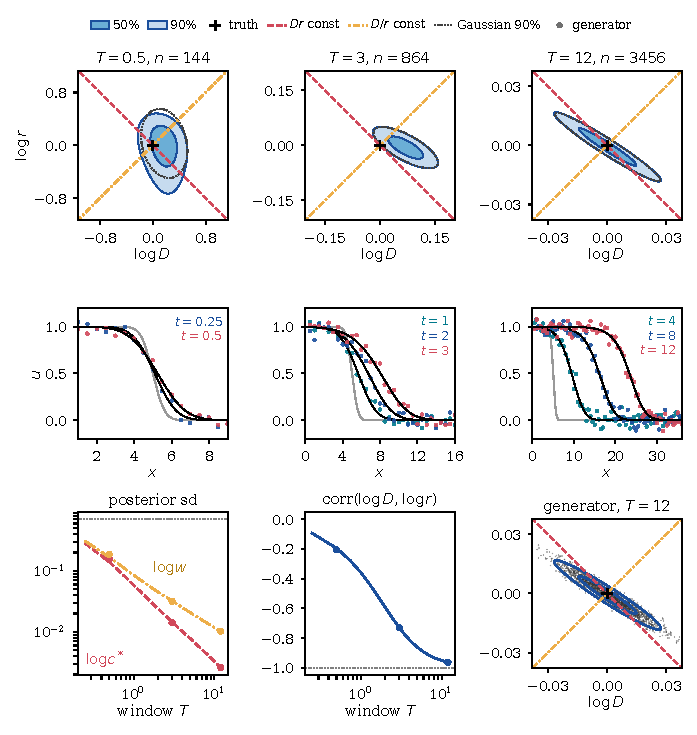
\includegraphics[width=\textwidth]{fk_posterior}
\caption{Exact posterior of $(\log D,\log r)$ for the Fisher Kolmogorov equation with $D=r=1$ and three nested observation windows $[0,T]$ with $n$ values; the axis scales differ. Top: $50$ and $90$ percent highest posterior density regions, the truth, the curves $Dr=\mathrm{const}$ (front speed) and $D/r=\mathrm{const}$ (front width) through it, and the $90$ percent region of the Gaussian approximation at the posterior mode (dotted). Middle: data (dots), solution at the posterior mean (black) and initial condition (gray). Bottom: posterior standard deviations of $\log c^*$ and $\log w$, with $c^*=2\sqrt{rD}$ and $w=\sqrt{D/r}$, and correlation of $(\log D,\log r)$ from the linearization at the truth as the window grows, with the exact values at the three windows (dots) and the prior standard deviation of $\log c^*$ and $\log w$ (dotted line); and $2000$ draws of a generator trained on $20000$ simulations, with the exact contours, for $T=12$.}
\label{fig:fk_posterior}
\end{figure}

\begin{table}[t]\centering\small
\caption{Exact posterior of $(\log D,\log r)$ by observation window: standard deviations $\sigma_D$ and $\sigma_r$ of $\log D$ and $\log r$, their correlation $\rho$, the ratio of the lengths of the principal axes of the contours, the angle of the long axis from the $\log D$ axis in degrees ($135$ is the curve $Dr=\mathrm{const}$ and $45$ the curve $D/r=\mathrm{const}$), and the standard deviations $\sigma_c$ and $\sigma_w$ of $\log c^*$ and $\log w$. The prior standard deviation of $\log D$ and $\log r$ is $1$.}\label{tab:fk_posterior}
\begin{tabular}{rrrrrrrr}
\toprule
$T$ & $\sigma_D$ & $\sigma_r$ & $\rho$ & ratio & angle & $\sigma_c$ & $\sigma_w$\\
\midrule
$0.5$ & $0.170$ & $0.298$ & $-0.21$ & $1.8$ & $100$ & $0.156$ & $0.186$\\
$3$ & $0.0412$ & $0.0263$ & $-0.73$ & $2.9$ & $151$ & $0.0142$ & $0.0315$\\
$12$ & $0.0125$ & $0.0081$ & $-0.96$ & $8.1$ & $147$ & $0.0026$ & $0.0103$\\
\bottomrule
\end{tabular}
\end{table}


\section{Two dimensional Navier Stokes on the torus}

In two dimensions the vorticity $\omega = \partial_1u_2-\partial_2u_1$ satisfies
\[
\partial_t\omega+u\cdot\nabla\omega = \nu\Delta\omega+\mathrm{curl}\,f,\qquad u = \nabla^\perp\Delta^{-1}\omega.
\]
The enstrophy $\int\omega^2$ is nonincreasing without forcing, which gives global regularity. The inverse problem of recovering $\omega(0)$ from noisy observations of $\omega(T)$ inherits the logarithmic instability of the heat equation at high frequencies, but the nonlinearity transfers energy between modes, so that information about one mode is partially encoded in others, and the posterior is no longer diagonal, as the computed example of Section~\ref{sec:simns2d} shows. As in the linear case, the posterior concentrates on large scale vortex structures and leaves small scales close to the prior in that example (Figure~\ref{fig:ns2d_posterior}). The theorems are proved for a different observation scheme. When the observations are spread over space and time starting at time zero, the information operator differs from that of the heat equation by a compact operator, smooth functionals of the state at a fixed later time have Gaussian limits at the rate $N^{-1/2}$ by the delta method, the energy and the circulation around a loop being examples, and credible bands for the trajectory have asymptotically exact coverage~\cite{konennickl2026}. The posterior can be computed by a generator trained on simulations, but the accuracy that the Gaussian statements need from the generator is a hypothesis and not a theorem (Proposition~\ref{prop:bvm_generators}). In the nonlinear experiment of Section~\ref{m:sec:expns}, a six mode truncation of the vorticity equation observed at $80$ points of space and time, a generator with an identity head trained on simulations from the prior stayed about one posterior standard deviation from a Metropolis reference as the number of simulations grew, and a generator trained near a preliminary estimate, with its residuals centered and rescaled, came to about $0.07$ posterior standard deviations~\cite{polsonsokolov2026manifold}. That is the accuracy of the Laplace approximation at the posterior mode, within the Monte Carlo error of the reference. The case for the generator in this experiment is amortization, not accuracy.

\section{History: filtering, calibration and assimilation}

Bayesian inference for dynamical systems has a long history in statistics and in the geosciences, developed largely independently. Carlin, Polson and Stoffer~\cite{cps1992} introduced Gibbs sampling for nonlinear and non Gaussian state space models. Polson and Roberts~\cite{polsonroberts1994} gave Bayes factors for diffusions observed at discrete times. Polson and Stroud developed simulation based inference for derivative pricing models, and the practical filter of Polson, Stroud and M\"uller~\cite{psm2008} addressed sequential parameter learning. Kennedy and O'Hagan~\cite{kennedyohagan2001} formalized the calibration of computer models with Gaussian process emulators and a model discrepancy term, and Higdon and coauthors extended the approach to high dimensional outputs. In meteorology, four dimensional variational assimilation computes the maximum a posteriori initial condition for a Gaussian prior and likelihood using an adjoint model, and Evensen's ensemble Kalman filter~\cite{evensen1994} propagates an ensemble of states through the forecast model and updates it linearly. In the language of this book, four dimensional variational assimilation is the mode of the posterior on the solution manifold, the ensemble Kalman filter is an affine transport approximation to the posterior (Chapter~\ref{ch:gbc}), and generative Bayesian computation is its nonlinear completion.

\section{Gaussian measures on function spaces}

The priors of this chapter are Gaussian measures on infinite dimensional spaces. Let $\mu = N(0,\mathcal{C})$ be a centered Gaussian measure on a separable Hilbert space $H$ with trace class covariance $\mathcal{C}$. Its Cameron Martin space is $E = \mathcal{C}^{1/2}H$ with norm $\|h\|_E = \|\mathcal{C}^{-1/2}h\|_H$.

\begin{theorem}[Cameron Martin, Feldman and H\'ajek]
\label{thm:cameron_martin}
The shifted measure $\mu(\cdot-h)$ is equivalent to $\mu$ if $h\in E$ and mutually singular with it otherwise. For $h\in E$,
\[
\frac{\dd\mu(\cdot-h)}{\dd\mu}(x) = \exp\Big(\langle\mathcal{C}^{-1/2}h,\mathcal{C}^{-1/2}x\rangle-\frac12\|h\|_E^2\Big),
\]
where $\langle\mathcal{C}^{-1/2}h,\mathcal{C}^{-1/2}x\rangle$ is the Paley Wiener integral: the $L^2(\mu)$ limit of $\langle\mathcal{C}^{-1}h_n,x\rangle$ for any $h_n\in\mathcal{C}H$ with $h_n\to h$ in $E$. It is a centered Gaussian variable with variance $\|h\|_E^2$. Two Gaussian measures are either equivalent or mutually singular.
\end{theorem}

We quote the theorem without proof. The density is the Cameron Martin formula and the dichotomy is the Feldman H\'ajek theorem; both are proved in Bogachev~\cite{bogachev1998}.

The Cameron Martin space has $\mu$ measure zero in infinite dimensions: draws from the prior are rougher than the functions the prior considers typical shifts. The maximum a posteriori estimator is defined through the Onsager Machlup functional
\[
I(\theta) = \mathcal{V}(\theta;y)+\frac12\|\theta\|_E^2,\qquad\mathcal{V}(\theta;y) = \frac{1}{2\delta^2}\|y-\mathcal{G}(\theta)\|^2,
\]
whose minimizer over $E$ is the Tikhonov regularized solution with penalty given by the Cameron Martin norm. Dashti, Law, Stuart and Voss~\cite{dashti2013} proved that this minimizer is the limit of the centers of small balls of maximal posterior probability, which gives the maximum a posteriori estimator a measure theoretic meaning in infinite dimensions.

\section{Well posedness of the posterior}

\begin{theorem}[Stuart]
\label{thm:stuart_wellposed}
Let $\Pi$ be a probability measure on a separable Banach space $X$ and let $\mathcal{V}:X\times\R^m\to\R$ be continuous. Suppose that for every $r>0$ there are nondecreasing functions $M_1(r,\cdot)$ and $M_2(r,\cdot)$, with $M_2$ strictly positive, such that for all $\theta\in X$ and all $y,y_1,y_2\in\R^m$ of norm at most $r$,
\[
\begin{gathered}
\mathcal{V}(\theta;y)\geq-M_1(r,\|\theta\|),\\
|\mathcal{V}(\theta;y_1)-\mathcal{V}(\theta;y_2)|\leq M_2(r,\|\theta\|)\,\|y_1-y_2\|,
\end{gathered}
\]
and that, for every $r>0$, $e^{M_1(r,\|\theta\|)}\big(1+M_2(r,\|\theta\|)^2\big)$ is integrable under $\Pi$. Then $Z(y) = \int e^{-\mathcal{V}(\theta;y)}\Pi(\dd\theta)$ is positive and finite, the measure $\Pi^y$ with density $Z(y)^{-1}e^{-\mathcal{V}(\theta;y)}$ with respect to $\Pi$ is a probability measure, and for every $r>0$ there is $C$ such that
\[
d_{\mathrm{Hell}}\big(\Pi^y,\Pi^{y'}\big)\leq C\|y-y'\|
\]
for all $y,y'$ of norm at most $r$.
\end{theorem}

This is a special case of the well posedness theorems of Dashti and Stuart~\cite{dashti2017}. The theorem holds for data in a Banach space. For a Gaussian prior the integrability condition is checked with Fernique's theorem, which gives $\int e^{\varepsilon\|\theta\|^2}\Pi(\dd\theta)<\infty$ for small $\varepsilon>0$. The condition holds for the potential $\mathcal{V}(\theta;y) = \frac{1}{2\delta^2}\|y-\mathcal{G}(\theta)\|^2$ when $\mathcal{G}$ is continuous and grows at most polynomially in $\|\theta\|$, with $M_1 = 0$ and $M_2(r,s) = \delta^{-2}\big(r+\sup_{\|\theta\|\leq s}\|\mathcal{G}(\theta)\|\big)$.

\begin{proof}[Sketch]
Fix $r>0$ and write $M_i$ for $M_i(r,\|\theta\|)$. The lower bound gives $Z(y)\leq\int e^{M_1}\dd\Pi<\infty$. Take a point $\theta_0$ in the support of $\Pi$. By continuity and the Lipschitz bound in $y$, $\mathcal{V}$ is bounded above, uniformly for $\|y\|\leq r$, on a neighborhood of $\theta_0$, and the neighborhood has positive prior mass, so $Z(y)$ is bounded away from zero. For $a,b\geq-M$ one has $|e^{-a}-e^{-b}|\leq e^M|a-b|$ and $|e^{-a/2}-e^{-b/2}|\leq\frac12e^{M/2}|a-b|$. Hence
\[
\begin{gathered}
|Z(y)-Z(y')|\leq\|y-y'\|\int e^{M_1}M_2\,\dd\Pi,\\
\int\big(e^{-\mathcal{V}(\theta;y)/2}-e^{-\mathcal{V}(\theta;y')/2}\big)^2\,\dd\Pi\leq\frac14\|y-y'\|^2\int e^{M_1}M_2^2\,\dd\Pi,
\end{gathered}
\]
and both integrals are finite by assumption. The squared Hellinger distance is at most a constant times the sum of the second integral and $|Z(y)-Z(y')|^2$, with a constant that depends on the lower bound for $Z$, and the claim follows.
\end{proof}

The map from data to the least squares initial condition is discontinuous, since the backward heat equation is ill posed in Hadamard's sense, but the map from data to posterior is Lipschitz in the Hellinger metric. Bayesian inversion is well posed where deterministic inversion is not, because it returns a measure that spreads its mass over the directions the data cannot determine.

\section{Dimension robust sampling}\label{sec:dimrobust}

Standard random walk Metropolis algorithms degenerate as the discretization of a function space problem is refined: the acceptance rate falls to zero unless the step size shrinks with the dimension. The preconditioned Crank Nicolson proposal of Cotter, Roberts, Stuart and White~\cite{cotter2013} avoids this. With prior $N(0,\mathcal{C})$, propose
\[
\theta' = \sqrt{1-\beta^2}\,\theta+\beta\,\xi,\qquad\xi\sim N(0,\mathcal{C}),
\]
and accept with probability $\min\{1,\exp(\mathcal{V}(\theta;y)-\mathcal{V}(\theta';y))\}$. The proposal is reversible with respect to the prior, so the acceptance probability involves only the likelihood, and the algorithm is well defined on the infinite dimensional space. Hairer, Stuart and Vollmer~\cite{hairer2014} proved that for a large class of target measures its Wasserstein spectral gap is bounded below independently of the discretization, and that this gap implies a spectral gap in $L^2$. The algorithm is an instance of the general principle of this book: a Markov chain that preserves the reference measure exactly, here the Gaussian prior, and corrects only for the tilt, mirrors the structure of Gibbs conditioning, in which the reference measure is fixed and only the constraint changes.

\section{A simulated example in two dimensions}\label{sec:simns2d}

Figure~\ref{fig:ns2d} shows a pseudospectral solution of the two dimensional vorticity equation, started from ten Gaussian vortices of random sign and strength. Isolated vortices persist, vortices of opposite sign close to one another are sheared into filaments, and viscosity thins the filaments. Kraichnan, Leith and Batchelor~\cite{kraichnan1967,leith1968,batchelor1969} predicted that in two dimensions energy moves to large scales and enstrophy to small scales, a dual cascade. The lower panels of the figure show the energy and enstrophy spectra, summed over shells of the wavenumber (the caption gives the definition). They show the two directions of the dual cascade only in part within $t=5$. The energy at $k=1$ rises from $0.0265$ to $0.0315$, which viscosity alone cannot do, while the total energy falls by $11$ percent, and the share of the energy at $k\le3$ rises from $0.82$ to $0.87$, so energy moves to large scales. The share of the enstrophy at $k\ge16$ grows from $5\times10^{-7}$ to $2.4\times10^{-3}$, so some enstrophy moves to small scales, but the total enstrophy falls by $32$ percent and its mean wavenumber does not rise, from $3.9$ to $3.8$. Three times of one flow do not show an inertial range.

\begin{figure}[t]
\centering
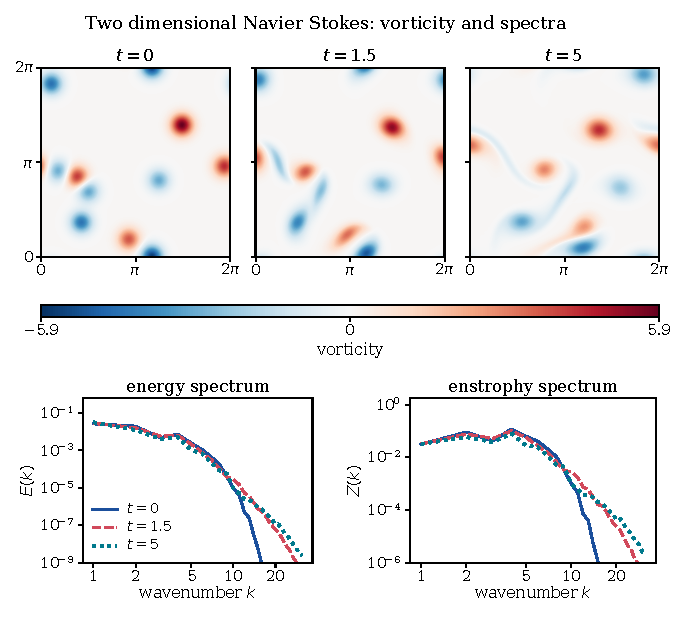
\includegraphics{ns2d}
\caption{Top: vorticity of a two dimensional Navier Stokes flow on the torus $[0,2\pi]^2$ with viscosity $\nu = 2\times10^{-3}$ at times $t = 0$, $1.5$ and $5$, started from ten Gaussian vortices of random sign. Red is positive and blue is negative vorticity (both print dark in grayscale), on one symmetric color scale for the three panels, with limits $\pm5.87$, the largest absolute value of the initial vorticity. Bottom: the energy spectrum $E(k)$ and the enstrophy spectrum $Z(k)$ per unit area at the same times, on logarithmic axes; with $\hat\omega_j$ the Fourier coefficients of the vorticity, $E(k)$ is the sum of $\frac12|\hat\omega_j|^2/|j|^2$ and $Z(k)$ the sum of $\frac12|\hat\omega_j|^2$ over the wavenumbers $j$ with $|j|$ rounded to $k$. The solution is computed by a dealiased pseudospectral method with fourth order Runge Kutta time stepping on a $96\times96$ grid.}
\label{fig:ns2d}
\end{figure}

We computed the inverse problem for a smaller flow than the one of Figure~\ref{fig:ns2d}, with a coarser grid and a larger viscosity, so that the posterior could be sampled exactly. The unknown is the initial vorticity $\omega_0=\sum_{0<|k|_\infty\le6}c_ke^{ik\cdot x}$ on $\T^2$, with $c_{-k}=\bar c_k$, which has $168$ real coefficients. The prior makes the coefficients independent and Gaussian with $\E|c_k|^2=(1+|k|^2)^{-2}$, a Mat\'ern type prior of smoothness index $1$ whose pointwise standard deviation is $1.47$. The data are the values of $\omega(T)$ at time $T=3$ at $16\times16$ equally spaced sensors, with independent Gaussian noise of standard deviation $\delta=0.25$, for viscosity $\nu=0.01$. The forward map is a dealiased pseudospectral solver with fourth order Runge Kutta steps of size $0.025$ on a $32\times32$ grid. The truth is five Gaussian vortices $a\,e^{-r^2/0.5}$, with amplitudes $a$ of both signs between $2.5$ and $6$ in absolute value, projected on the $168$ modes (Figure~\ref{fig:ns2d_posterior_data}), so that the model is correctly specified. The data were generated on a $64\times64$ grid with half the time step, not on the grid of the posterior, so that there is no inverse crime: the two solutions differ at the sensors by $0.03$ in root mean square, one ninth of $\delta$.

\begin{figure}[t]
\centering
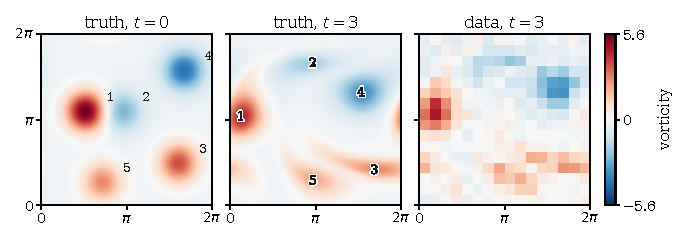
\includegraphics{ns2d_posterior_data}
\caption{Truth and data of the simulated inverse problem. Left: the initial vorticity of the truth, five Gaussian vortices numbered $1$ to $5$. Middle: the truth at the observation time $t=3$; the numbers mark where the five vortices have gone. Right: the data. One color scale for the three panels.}
\label{fig:ns2d_posterior_data}
\end{figure}

We found the maximum of the posterior density by a Levenberg Marquardt iteration, formed the Gauss Newton Hessian there, and sampled the posterior exactly by Hamiltonian Monte Carlo~\cite{duane1987,neal2011} in coordinates in which that Hessian is the identity. The gradient of the log posterior is the reverse mode derivative of the solver. Four chains were started from independent draws of the prior, and each ran $400$ warmup iterations, with the step size set by dual averaging~\cite{hoffman2014}, followed by $1000$ iterations with a random number of leapfrog steps. The mean acceptance probability was $0.77$. The largest rank normalized split $\widehat R$~\cite{vehtari2021} over the $168$ coefficients is $1.010$, and the smallest bulk effective sample size is $552$ out of $4000$ draws. The four chains reach the same posterior, and three further optimizations started from other prior draws end at the same maximum, so that we found no sign of several modes. That says nothing about regimes with a lower viscosity, a longer observation time or fewer sensors, which we did not compute. On the linear problem obtained by dropping the nonlinear term, whose posterior is Gaussian and known in closed form, the same sampler, with four chains of $300$ warmup and $600$ retained iterations, has $\widehat R\le1.009$ and reproduces the standard deviations of all $168$ coefficients to within $6$ percent, the largest of $168$ Monte Carlo errors of about $2$ percent each.

\begin{figure}[t]
\centering
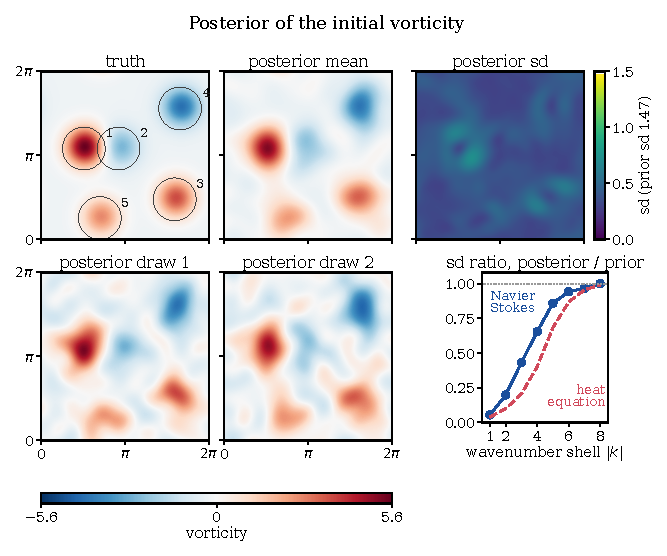
\includegraphics{ns2d_posterior}
\caption{Posterior of the initial vorticity for the data of Figure~\ref{fig:ns2d_posterior_data}, from four Hamiltonian Monte Carlo chains. Top: the truth, with the five discs of radius $0.8$ on which circulations are computed, the posterior mean, and the pointwise posterior standard deviation on a color scale from zero to the prior standard deviation $1.47$. Bottom: two posterior draws on the color scale of the truth, and the ratio of posterior to prior standard deviation of the Fourier coefficients by wavenumber shell (the square root of the ratio of the summed variances over the modes with $|k|$ rounded to $m$), for the nonlinear problem and for the problem with the nonlinear term dropped.}
\label{fig:ns2d_posterior}
\end{figure}

Figure~\ref{fig:ns2d_posterior} shows the posterior. The posterior mean recovers the five vortices, the draws differ from it in a fine scale texture that the data do not constrain, and the standard deviation of the field is at most $0.74$, against $1.47$ for the prior. By wavenumber shell, the ratio of the posterior to the prior standard deviation of the coefficients, pooled over the shell as in the caption, is $0.05$, $0.20$ and $0.43$ for $|k|=1,2,3$, $0.65$ at $|k|=4$ and $0.86$ at $|k|=5$, and at least $0.94$ for $|k|\ge6$: the large scales are learned and the small scales are left at the prior. With the nonlinear term dropped, the vorticity equation becomes the heat equation, and the same prior, sensors and noise give a diagonal posterior that learns more at every wavenumber, with ratios $0.04$, $0.10$, $0.20$, $0.40$ and $0.68$ for $|k|=1,\dots,5$. The nonlinear posterior is not diagonal: $158$ of the $14028$ pairs of coefficients have a posterior correlation above $0.3$ in absolute value, and the largest is $0.67$.

\begin{table}[t]\centering\footnotesize\setlength{\tabcolsep}{5pt}
\caption{Posterior mean and standard deviation (sd) of the energy and of the circulations of the initial vorticity. The prior standard deviation is $14.3$ for the energy, estimated from $20000$ prior draws, and $2.36$ for every circulation. The circulation is the integral of $\omega_0$ over the disc of radius $0.8$ around vortex $j$. The position error is the root mean square distance, over posterior draws, between the location of the extremum of $\omega_0$ in that disc and its location in the truth; under the prior it is between $0.72$ and $0.73$ for every vortex. The elongation is the ratio of the principal axes of the region in which vortex $j$, advected to $t=3$ separately by the velocity of the whole field, exceeds a fifth of its maximum; it is $1$ at $t=0$.}\label{tab:ns2d_posterior}
\begin{tabular}{@{}lrrrrr@{}}
\toprule
Functional & Truth & Mean & Sd & Position error & Elongation\\
\midrule
Energy & $12.62$ & $13.03$ & $0.42$ & & \\
Circulation 1 & $5.88$ & $5.78$ & $0.19$ & $0.14$ & $1.33$\\
Circulation 2 & $-2.37$ & $-2.39$ & $0.24$ & $0.32$ & $2.43$\\
Circulation 3 & $4.02$ & $3.85$ & $0.19$ & $0.20$ & $4.52$\\
Circulation 4 & $-5.06$ & $-5.03$ & $0.16$ & $0.26$ & $1.31$\\
Circulation 5 & $2.88$ & $2.70$ & $0.16$ & $0.26$ & $2.17$\\
\bottomrule
\end{tabular}
\end{table}

Table~\ref{tab:ns2d_posterior} gives the posterior of the energy $\frac12\int_{\T^2}|u_0|^2\dd x$ of the initial velocity and of the circulations on the discs of Figure~\ref{fig:ns2d_posterior}. The standard deviation of the energy is $3$ percent of its prior value and those of the circulations are $7$ to $10$ percent of theirs. The truth is within $1.2$ posterior standard deviations of the posterior mean for each of the six, and the posterior of the energy is close to normal, with skewness $0.10$ and excess kurtosis $-0.03$. We repeated the computation with the same noise draw rescaled to $\delta=0.5$ and $\delta=0.125$, with $300$ warmup and $600$ retained iterations per chain, $\widehat R\le1.03$ and a bulk effective sample size of at least $196$ for the coordinates; the Monte Carlo error of each standard deviation of a functional below is $2$ to $4$ percent. The standard deviation of the energy is $0.83$, $0.42$ and $0.21$ for $\delta=0.5$, $0.25$ and $0.125$, proportional to $\delta$ within $2$ percent, and those of the circulations of vortices 1, 3, 4 and 5 scale as $\delta^s$ over the same range with $s$ between $0.90$ and $1.07$. The circulation of vortex 2, the weakest, scales as $\delta^{0.73}$, and the point value of $\omega_0$ at the center of vortex 1, which depends on small scales, as $\delta^{0.68}$. A standard deviation proportional to $\delta$, together with a nearly normal posterior, is what a Bernstein von Mises theorem leads one to expect of a smooth functional. In this experiment the energy has both. One experiment says nothing about rates. The Gaussian approximation at the maximum of the posterior gives standard deviations of these six functionals that are $4$ to $11$ percent too small, and the importance weights of its draws have an effective sample size of $0.9$ percent, so that as a measure on $\R^{168}$ it is not close to the posterior.

The five vortices are not determined equally well. Advected separately by the velocity of the whole field, vortices 3 and 5 are drawn by $t=3$ into thin arcs and vortex 2 into a flat band, while vortices 1 and 4 stay compact (Table~\ref{tab:ns2d_posterior}). The standard deviation of the circulation of vortex 2 is the largest of the five, and so is the error of its position. But vortex 3, the most elongated, has the circulation standard deviation of the compact vortex 1, and vortex 5, which is also drawn into an arc, has a circulation standard deviation as small as that of the compact vortex 4. Vortex 2 is also the weakest of the five, so that this experiment shows no clear effect of filamentation on how well a vortex is determined.


\section*{Exercises}
\begin{enumerate}
\item In the heat equation sequence model, derive the posterior mean and variance of $\theta_k$.
\item Show that the functional $L\theta = \theta_1$ satisfies the summability condition of Theorem~\ref{thm:heat_rates} and compute its asymptotic variance.
\item Prove that the preconditioned Crank Nicolson proposal is reversible with respect to $N(0,\mathcal{C})$.
\item Show that a traveling front $U(x-ct)$ of the Fisher Kolmogorov equation satisfies $DU''+cU'+rU(1-U) = 0$, and that rescaling the variable by $\sqrt{D/r}$ leaves the single parameter $c/\sqrt{rD}$.
\item Compute the Cameron Martin norm of a smooth function $h$ with $h(0) = 0$ under the Brownian motion prior on $[0,1]$.
\end{enumerate}


\section*{Notes}

The generative computation on the solution manifold is from our paper~\cite{polsonsokolov2026manifold}. Our earlier paper~\cite{polsonsokolov2026ns} treats the discretized Navier Stokes equations as a state space model and learns parameters by particle learning.
